%!TEX root = ./main.tex



\tikzset{every picture/.style={line width=0.75pt}} %set default line width to 0.75pt        

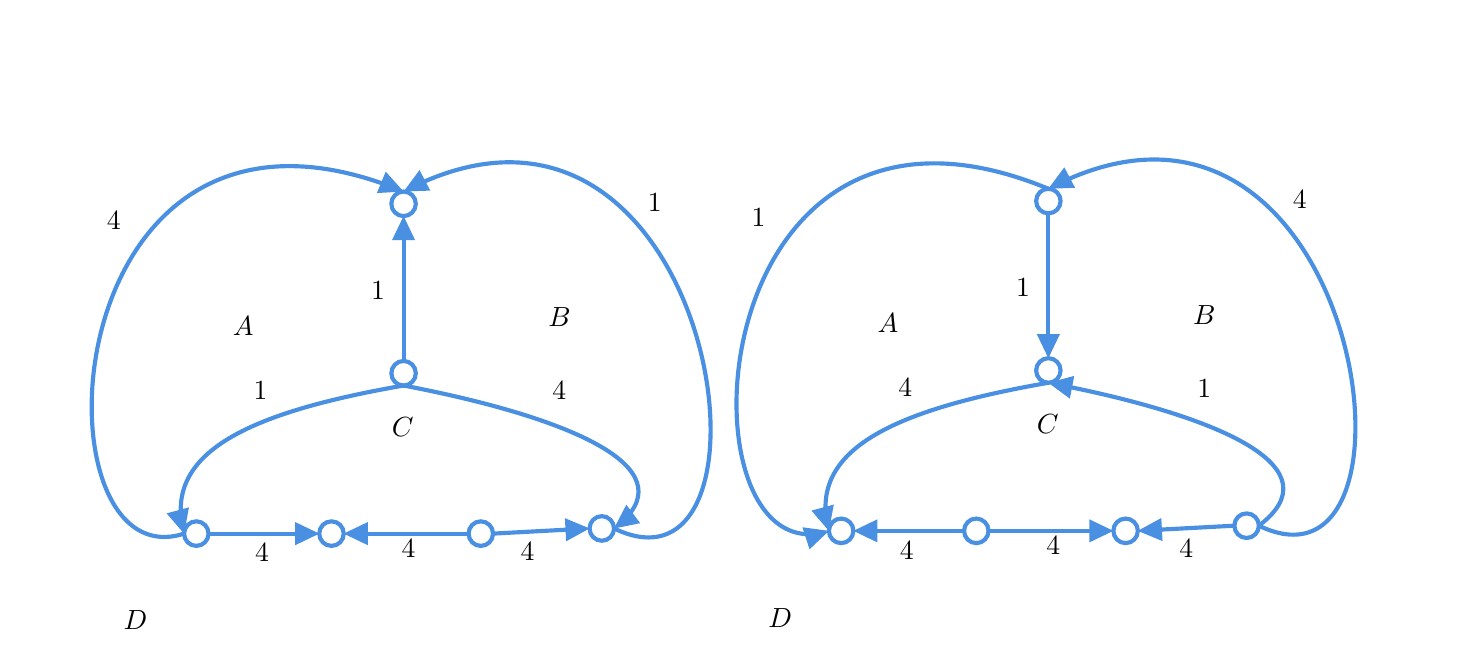
\begin{tikzpicture}[x=0.75pt,y=0.75pt,yscale=-1,xscale=1]
%uncomment if require: \path (0,877); %set diagram left start at 0, and has height of 877

%Shape: Ellipse [id:dp2062482206131232] 
\draw  [color={rgb, 255:red, 74; green, 144; blue, 226 }  ,draw opacity=1 ][line width=1.5]  (181.18,43.69) .. controls (181.18,40.42) and (183.82,37.77) .. (187.08,37.77) .. controls (190.33,37.77) and (192.97,40.42) .. (192.97,43.69) .. controls (192.97,46.95) and (190.33,49.6) .. (187.08,49.6) .. controls (183.82,49.6) and (181.18,46.95) .. (181.18,43.69) -- cycle ;
%Shape: Ellipse [id:dp42181631305663214] 
\draw  [color={rgb, 255:red, 74; green, 144; blue, 226 }  ,draw opacity=1 ][line width=1.5]  (181.18,125.31) .. controls (181.18,122.05) and (183.82,119.39) .. (187.08,119.39) .. controls (190.33,119.39) and (192.97,122.05) .. (192.97,125.31) .. controls (192.97,128.58) and (190.33,131.23) .. (187.08,131.23) .. controls (183.82,131.23) and (181.18,128.58) .. (181.18,125.31) -- cycle ;
%Shape: Ellipse [id:dp1893981875046039] 
\draw  [color={rgb, 255:red, 74; green, 144; blue, 226 }  ,draw opacity=1 ][line width=1.5]  (81.33,202.58) .. controls (81.33,199.31) and (83.97,196.66) .. (87.22,196.66) .. controls (90.48,196.66) and (93.11,199.31) .. (93.11,202.58) .. controls (93.11,205.85) and (90.48,208.5) .. (87.22,208.5) .. controls (83.97,208.5) and (81.33,205.85) .. (81.33,202.58) -- cycle ;
%Shape: Ellipse [id:dp3630097335542829] 
\draw  [color={rgb, 255:red, 74; green, 144; blue, 226 }  ,draw opacity=1 ][line width=1.5]  (276.69,200.09) .. controls (276.69,196.82) and (279.33,194.17) .. (282.59,194.17) .. controls (285.84,194.17) and (288.48,196.82) .. (288.48,200.09) .. controls (288.48,203.36) and (285.84,206.01) .. (282.59,206.01) .. controls (279.33,206.01) and (276.69,203.36) .. (276.69,200.09) -- cycle ;
%Shape: Ellipse [id:dp12213112120599945] 
\draw  [color={rgb, 255:red, 74; green, 144; blue, 226 }  ,draw opacity=1 ][line width=1.5]  (146.45,202.58) .. controls (146.45,199.31) and (149.09,196.66) .. (152.34,196.66) .. controls (155.6,196.66) and (158.24,199.31) .. (158.24,202.58) .. controls (158.24,205.85) and (155.6,208.5) .. (152.34,208.5) .. controls (149.09,208.5) and (146.45,205.85) .. (146.45,202.58) -- cycle ;
%Shape: Ellipse [id:dp14956651149377553] 
\draw  [color={rgb, 255:red, 74; green, 144; blue, 226 }  ,draw opacity=1 ][line width=1.5]  (218.4,202.58) .. controls (218.4,199.31) and (221.03,196.66) .. (224.29,196.66) .. controls (227.54,196.66) and (230.18,199.31) .. (230.18,202.58) .. controls (230.18,205.85) and (227.54,208.5) .. (224.29,208.5) .. controls (221.03,208.5) and (218.4,205.85) .. (218.4,202.58) -- cycle ;
%Curve Lines [id:da46118430818328493] 
\draw [color={rgb, 255:red, 74; green, 144; blue, 226 }  ,draw opacity=1 ][line width=1.5]    (80.43,198.63) .. controls (73.79,162.96) and (112.86,144.16) .. (187.08,131.23) ;
\draw [shift={(81.33,202.58)}, rotate = 254.88] [fill={rgb, 255:red, 74; green, 144; blue, 226 }  ,fill opacity=1 ][line width=0.08]  [draw opacity=0] (11.61,-5.58) -- (0,0) -- (11.61,5.58) -- cycle    ;
%Curve Lines [id:da12684350601217753] 
\draw [color={rgb, 255:red, 74; green, 144; blue, 226 }  ,draw opacity=1 ][line width=1.5]    (292.05,197.16) .. controls (321.77,170.32) and (267.27,146.57) .. (187.08,131.23) ;
\draw [shift={(288.48,200.09)}, rotate = 323] [fill={rgb, 255:red, 74; green, 144; blue, 226 }  ,fill opacity=1 ][line width=0.08]  [draw opacity=0] (11.61,-5.58) -- (0,0) -- (11.61,5.58) -- cycle    ;
%Curve Lines [id:da12533726813089074] 
\draw [color={rgb, 255:red, 74; green, 144; blue, 226 }  ,draw opacity=1 ][line width=1.5]    (288.48,200.09) .. controls (375.8,242.25) and (338.78,-38.85) .. (189.34,36.6) ;
\draw [shift={(187.08,37.77)}, rotate = 332.3] [fill={rgb, 255:red, 74; green, 144; blue, 226 }  ,fill opacity=1 ][line width=0.08]  [draw opacity=0] (11.61,-5.58) -- (0,0) -- (11.61,5.58) -- cycle    ;
%Curve Lines [id:da052098391594170956] 
\draw [color={rgb, 255:red, 74; green, 144; blue, 226 }  ,draw opacity=1 ][line width=1.5]    (81.33,202.58) .. controls (6.97,226.76) and (15.81,-30.37) .. (184.52,36.73) ;
\draw [shift={(187.08,37.77)}, rotate = 202.45] [fill={rgb, 255:red, 74; green, 144; blue, 226 }  ,fill opacity=1 ][line width=0.08]  [draw opacity=0] (11.61,-5.58) -- (0,0) -- (11.61,5.58) -- cycle    ;
%Straight Lines [id:da025851980169662614] 
\draw [color={rgb, 255:red, 74; green, 144; blue, 226 }  ,draw opacity=1 ][line width=1.5]    (93.11,202.58) -- (142.45,202.58) ;
\draw [shift={(146.45,202.58)}, rotate = 180] [fill={rgb, 255:red, 74; green, 144; blue, 226 }  ,fill opacity=1 ][line width=0.08]  [draw opacity=0] (11.61,-5.58) -- (0,0) -- (11.61,5.58) -- cycle    ;
%Straight Lines [id:da7108101232087555] 
\draw [color={rgb, 255:red, 74; green, 144; blue, 226 }  ,draw opacity=1 ][line width=1.5]    (162.24,202.58) -- (218.4,202.58) ;
\draw [shift={(158.24,202.58)}, rotate = 0] [fill={rgb, 255:red, 74; green, 144; blue, 226 }  ,fill opacity=1 ][line width=0.08]  [draw opacity=0] (11.61,-5.58) -- (0,0) -- (11.61,5.58) -- cycle    ;
%Straight Lines [id:da4593573245399082] 
\draw [color={rgb, 255:red, 74; green, 144; blue, 226 }  ,draw opacity=1 ][line width=1.5]    (230.18,202.58) -- (272.7,200.3) ;
\draw [shift={(276.69,200.09)}, rotate = 176.93] [fill={rgb, 255:red, 74; green, 144; blue, 226 }  ,fill opacity=1 ][line width=0.08]  [draw opacity=0] (11.61,-5.58) -- (0,0) -- (11.61,5.58) -- cycle    ;
%Straight Lines [id:da3678344551576813] 
\draw [color={rgb, 255:red, 74; green, 144; blue, 226 }  ,draw opacity=1 ][line width=1.5]    (187.08,119.39) -- (187.08,53.6) ;
\draw [shift={(187.08,49.6)}, rotate = 90] [fill={rgb, 255:red, 74; green, 144; blue, 226 }  ,fill opacity=1 ][line width=0.08]  [draw opacity=0] (11.61,-5.58) -- (0,0) -- (11.61,5.58) -- cycle    ;
%Shape: Ellipse [id:dp5834798930697471] 
\draw  [color={rgb, 255:red, 74; green, 144; blue, 226 }  ,draw opacity=1 ][line width=1.5]  (491.85,42.35) .. controls (491.85,39.08) and (494.49,36.43) .. (497.74,36.43) .. controls (501,36.43) and (503.63,39.08) .. (503.63,42.35) .. controls (503.63,45.62) and (501,48.27) .. (497.74,48.27) .. controls (494.49,48.27) and (491.85,45.62) .. (491.85,42.35) -- cycle ;
%Shape: Ellipse [id:dp9667981945481139] 
\draw  [color={rgb, 255:red, 74; green, 144; blue, 226 }  ,draw opacity=1 ][line width=1.5]  (491.85,123.98) .. controls (491.85,120.71) and (494.49,118.06) .. (497.74,118.06) .. controls (501,118.06) and (503.63,120.71) .. (503.63,123.98) .. controls (503.63,127.25) and (501,129.9) .. (497.74,129.9) .. controls (494.49,129.9) and (491.85,127.25) .. (491.85,123.98) -- cycle ;
%Shape: Ellipse [id:dp09059574964185924] 
\draw  [color={rgb, 255:red, 74; green, 144; blue, 226 }  ,draw opacity=1 ][line width=1.5]  (392,201.25) .. controls (392,197.98) and (394.64,195.33) .. (397.89,195.33) .. controls (401.14,195.33) and (403.78,197.98) .. (403.78,201.25) .. controls (403.78,204.52) and (401.14,207.17) .. (397.89,207.17) .. controls (394.64,207.17) and (392,204.52) .. (392,201.25) -- cycle ;
%Shape: Ellipse [id:dp3605131756242862] 
\draw  [color={rgb, 255:red, 74; green, 144; blue, 226 }  ,draw opacity=1 ][line width=1.5]  (587.36,198.76) .. controls (587.36,195.49) and (590,192.84) .. (593.25,192.84) .. controls (596.51,192.84) and (599.15,195.49) .. (599.15,198.76) .. controls (599.15,202.03) and (596.51,204.68) .. (593.25,204.68) .. controls (590,204.68) and (587.36,202.03) .. (587.36,198.76) -- cycle ;
%Shape: Ellipse [id:dp6418673252768715] 
\draw  [color={rgb, 255:red, 74; green, 144; blue, 226 }  ,draw opacity=1 ][line width=1.5]  (457.12,201.25) .. controls (457.12,197.98) and (459.76,195.33) .. (463.01,195.33) .. controls (466.27,195.33) and (468.9,197.98) .. (468.9,201.25) .. controls (468.9,204.52) and (466.27,207.17) .. (463.01,207.17) .. controls (459.76,207.17) and (457.12,204.52) .. (457.12,201.25) -- cycle ;
%Shape: Ellipse [id:dp39805151621059387] 
\draw  [color={rgb, 255:red, 74; green, 144; blue, 226 }  ,draw opacity=1 ][line width=1.5]  (529.06,201.25) .. controls (529.06,197.98) and (531.7,195.33) .. (534.95,195.33) .. controls (538.21,195.33) and (540.85,197.98) .. (540.85,201.25) .. controls (540.85,204.52) and (538.21,207.17) .. (534.95,207.17) .. controls (531.7,207.17) and (529.06,204.52) .. (529.06,201.25) -- cycle ;
%Curve Lines [id:da1957524342127539] 
\draw [color={rgb, 255:red, 74; green, 144; blue, 226 }  ,draw opacity=1 ][line width=1.5]    (391.09,197.3) .. controls (384.45,161.63) and (423.53,142.83) .. (497.74,129.9) ;
\draw [shift={(392,201.25)}, rotate = 254.88] [fill={rgb, 255:red, 74; green, 144; blue, 226 }  ,fill opacity=1 ][line width=0.08]  [draw opacity=0] (11.61,-5.58) -- (0,0) -- (11.61,5.58) -- cycle    ;
%Curve Lines [id:da3321764957558633] 
\draw [color={rgb, 255:red, 74; green, 144; blue, 226 }  ,draw opacity=1 ][line width=1.5]    (599.15,198.76) .. controls (635.8,171.14) and (582.49,146.54) .. (501.46,130.62) ;
\draw [shift={(497.74,129.9)}, rotate = 10.82] [fill={rgb, 255:red, 74; green, 144; blue, 226 }  ,fill opacity=1 ][line width=0.08]  [draw opacity=0] (11.61,-5.58) -- (0,0) -- (11.61,5.58) -- cycle    ;
%Curve Lines [id:da2799756577005189] 
\draw [color={rgb, 255:red, 74; green, 144; blue, 226 }  ,draw opacity=1 ][line width=1.5]    (599.15,198.76) .. controls (686.47,240.92) and (649.45,-40.18) .. (500,35.27) ;
\draw [shift={(497.74,36.43)}, rotate = 332.3] [fill={rgb, 255:red, 74; green, 144; blue, 226 }  ,fill opacity=1 ][line width=0.08]  [draw opacity=0] (11.61,-5.58) -- (0,0) -- (11.61,5.58) -- cycle    ;
%Curve Lines [id:da9026596524821855] 
\draw [color={rgb, 255:red, 74; green, 144; blue, 226 }  ,draw opacity=1 ][line width=1.5]    (387.62,202.37) .. controls (317.7,215.29) and (329.99,-32.88) .. (497.74,36.43) ;
\draw [shift={(392,201.25)}, rotate = 161.99] [fill={rgb, 255:red, 74; green, 144; blue, 226 }  ,fill opacity=1 ][line width=0.08]  [draw opacity=0] (11.61,-5.58) -- (0,0) -- (11.61,5.58) -- cycle    ;
%Straight Lines [id:da29172929203159703] 
\draw [color={rgb, 255:red, 74; green, 144; blue, 226 }  ,draw opacity=1 ][line width=1.5]    (407.78,201.25) -- (457.12,201.25) ;
\draw [shift={(403.78,201.25)}, rotate = 0] [fill={rgb, 255:red, 74; green, 144; blue, 226 }  ,fill opacity=1 ][line width=0.08]  [draw opacity=0] (11.61,-5.58) -- (0,0) -- (11.61,5.58) -- cycle    ;
%Straight Lines [id:da23336632170754767] 
\draw [color={rgb, 255:red, 74; green, 144; blue, 226 }  ,draw opacity=1 ][line width=1.5]    (468.9,201.25) -- (525.06,201.25) ;
\draw [shift={(529.06,201.25)}, rotate = 180] [fill={rgb, 255:red, 74; green, 144; blue, 226 }  ,fill opacity=1 ][line width=0.08]  [draw opacity=0] (11.61,-5.58) -- (0,0) -- (11.61,5.58) -- cycle    ;
%Straight Lines [id:da7582939485718254] 
\draw [color={rgb, 255:red, 74; green, 144; blue, 226 }  ,draw opacity=1 ][line width=1.5]    (544.84,201.03) -- (587.36,198.76) ;
\draw [shift={(540.85,201.25)}, rotate = 356.93] [fill={rgb, 255:red, 74; green, 144; blue, 226 }  ,fill opacity=1 ][line width=0.08]  [draw opacity=0] (11.61,-5.58) -- (0,0) -- (11.61,5.58) -- cycle    ;
%Straight Lines [id:da2633005133934979] 
\draw [color={rgb, 255:red, 74; green, 144; blue, 226 }  ,draw opacity=1 ][line width=1.5]    (497.74,114.06) -- (497.74,48.27) ;
\draw [shift={(497.74,118.06)}, rotate = 270] [fill={rgb, 255:red, 74; green, 144; blue, 226 }  ,fill opacity=1 ][line width=0.08]  [draw opacity=0] (11.61,-5.58) -- (0,0) -- (11.61,5.58) -- cycle    ;

% Text Node
\draw (103.33,96.4) node [anchor=north west][inner sep=0.75pt]    {$A$};
% Text Node
\draw (255.33,92.4) node [anchor=north west][inner sep=0.75pt]    {$B$};
% Text Node
\draw (180,145.07) node [anchor=north west][inner sep=0.75pt]    {$C$};
% Text Node
\draw (50.67,238.4) node [anchor=north west][inner sep=0.75pt]    {$D$};
% Text Node
\draw (303.33,37.4) node [anchor=north west][inner sep=0.75pt]    {$1$};
% Text Node
\draw (113.33,127.73) node [anchor=north west][inner sep=0.75pt]    {$1$};
% Text Node
\draw (257.33,128.07) node [anchor=north west][inner sep=0.75pt]    {$4$};
% Text Node
\draw (42.67,46.07) node [anchor=north west][inner sep=0.75pt]    {$4$};
% Text Node
\draw (114,206.07) node [anchor=north west][inner sep=0.75pt]    {$4$};
% Text Node
\draw (184.67,204.07) node [anchor=north west][inner sep=0.75pt]    {$4$};
% Text Node
\draw (242,205.4) node [anchor=north west][inner sep=0.75pt]    {$4$};
% Text Node
\draw (170,79.73) node [anchor=north west][inner sep=0.75pt]    {$1$};
% Text Node
\draw (414,95.07) node [anchor=north west][inner sep=0.75pt]    {$A$};
% Text Node
\draw (566,91.07) node [anchor=north west][inner sep=0.75pt]    {$B$};
% Text Node
\draw (490.67,143.73) node [anchor=north west][inner sep=0.75pt]    {$C$};
% Text Node
\draw (361.33,237.07) node [anchor=north west][inner sep=0.75pt]    {$D$};
% Text Node
\draw (614,36.07) node [anchor=north west][inner sep=0.75pt]    {$4$};
% Text Node
\draw (424,126.4) node [anchor=north west][inner sep=0.75pt]    {$4$};
% Text Node
\draw (568,126.73) node [anchor=north west][inner sep=0.75pt]    {$1$};
% Text Node
\draw (353.33,44.73) node [anchor=north west][inner sep=0.75pt]    {$1$};
% Text Node
\draw (424.67,204.73) node [anchor=north west][inner sep=0.75pt]    {$4$};
% Text Node
\draw (495.33,202.73) node [anchor=north west][inner sep=0.75pt]    {$4$};
% Text Node
\draw (559.33,204.07) node [anchor=north west][inner sep=0.75pt]    {$4$};
% Text Node
\draw (480.67,78.4) node [anchor=north west][inner sep=0.75pt]    {$1$};


\end{tikzpicture}